\documentclass[10pt]{mypackage}

% sans serif font:
%\usepackage{cmbright}
%\usepackage{sfmath}
%\usepackage{bbold} %better blackboard bold

%serif font + different blackboard bold for serif font
\usepackage{newpxtext,eulerpx}
\renewcommand*{\mathbb}[1]{\varmathbb{#1}}

%\usepackage{mathrsfs}
%\usetikzlibrary{arrows}
\pagestyle{fancy}
\fancyhf{}
\rhead{Avinash Iyer}
\lhead{Ordinary Differential Equations: Class Notes}

\setcounter{secnumdepth}{0}

\begin{document}
\section{First-Order Differential Equations}%
\subsection{Introduction to First-Order Differential Equations}%
  Recall that for $y = f(x)$, $x$ is the independent variable and $y$ is the dependent variable.
  \begin{definition}[Differential Equation]
  A differential equation is an equation which contains derivatives of a dependent variable with respect to one or more independent variables.
  \end{definition}
  \begin{example}[A Basic Differential Equation]
    \begin{align*}
      \frac{dy}{dx} - 5y - 1 &= 0
    \end{align*}
  \end{example}
  We can classify differential equations by
  \begin{itemize}
    \item type;
    \item order;
    \item linearity.
  \end{itemize}
  \begin{definition}[Classification by Type]
  There are two types of differential equations:
  \begin{itemize}
    \item ordinary differential equations (ODEs);
    \item partial differential equations (PDEs).
  \end{itemize}
  ODEs are characterized by derivatives of the dependent variable with respect to one independent variable. PDEs are characterized by derivatives of the dependent variable with respect to multiple independent variables.
  \end{definition}
  \begin{example}[ODEs and PDEs]\hfill
    \begin{enumerate}[(1)]
      \item An ODE:
        \begin{align*}
          \frac{d^2y}{dx^2} - 2\frac{dy}{dx} + 6y &= 0
        \end{align*}
      \item A PDE:
        \begin{align*}
          \pd{^2u}{x^2} + \pd{^2u}{y^2} &= 0
        \end{align*}
    \end{enumerate}
  \end{example}
  \begin{definition}[Classificiation by Order]
    The order of the highest derivative in a differential equation is the order of the differential equation.
  \end{definition}
  \begin{example}[Differential Equations of Varying Orders]\hfill
    \begin{enumerate}[(1)]
      \item 
        \begin{align*}
          \diff{^2y}{x^2} + 5\left(\frac{dy}{dx}\right) - 4y &= x \tag*{order 2}
        \end{align*}
      \item 
        \begin{align*}
          2\frac{dy}{dx} + y &= 0\tag*{order 1}
        \end{align*}
      \item 
        \begin{align*}
          \sin(x)y''' - \left(\cos x\right)y' &= 2\tag*{order 3}
        \end{align*}
    \end{enumerate}
  \end{example}
  In general, we write a differential equation of order $n$ in the form
  \begin{align*}
    \underbrace{F\left(x,y,\frac{dy}{dx},\frac{d^2y}{dx^2},\dots,\frac{d^ny}{dx^n}\right)}_{\text{$n+2$ variables}} = 0.
  \end{align*}
  \begin{example}
    Suppose we have the differential equation
    \begin{align*}
      \frac{d^3y}{dx^3} + y^2 &= x.
    \end{align*}
    Then, we rewrite as
    \begin{align*}
      \underbrace{\frac{d^3y}{dx^3} + y^2 - x}_{F\left(x,y,\frac{dx}{dy},\frac{d^2x}{dy^2},\frac{d^3x}{dy^3}\right)} &= 0.
    \end{align*}
    Alternatively, we can write as
    \begin{align*}
      \frac{d^3y}{dx^3} &= \underbrace{x - y^2}_{f(x,y)}.
    \end{align*}
  \end{example}
  \begin{definition}[Classification by Linearity]
    We much prefer to analyze linear differential equations over nonlinear differential equations.\newline

    A differential equation is linear if it has the following form:
    \begin{align*}
      a_n(x)\frac{d^ny}{dx^n} + a_{n-1}(x)\frac{d^{n-1}y}{dx^{n-1}} + \cdots + a_{1}(x)\frac{dy}{dx} + a_0(x)y &= g(x).
    \end{align*}
    \begin{enumerate}[(1)]
      \item The power of each term involving $y$ and all its derivatives is one.
      \item All coefficients are exclusively functions of $x$.
    \end{enumerate}
    A differential equation that is not linear is called nonlinear.
  \end{definition}
  \begin{example}[Linear Differential Equations (or lack thereof)]\hfill
    \begin{enumerate}[(1)]
      \item 
        \begin{align*}
          x^3\frac{d^3y}{dx^3} - x^2\frac{d^2y}{dx^2} + 3x\frac{dy}{dx} + 5y &= e^x \tag*{Linear}
        \end{align*}
      \item 
        \begin{align*}
          yy'' - 2y' &= x\tag*{Nonlinear}
        \end{align*}
      \item 
        \begin{align*}
          \frac{d^3y}{dx^3} + y^2 &= 0 \tag*{Nonlinear}
        \end{align*}
    \end{enumerate}
  \end{example}
  \begin{definition}[Autonomous Differential Equations]
    An autonomous (first-order) differential equation is a differential equation in the following form:
    \begin{align*}
      \frac{dy}{dx} &= f(y).
    \end{align*}
  \end{definition}
  \begin{definition}[Solution to an ODE]
    Consider the general ODE
    \begin{align*}
      F\left(x,y,\frac{dy}{dx},\frac{d^2y}{dx^2},\dots,\frac{d^ny}{dx^n}\right) &= 0.\tag*{(\textasteriskcentered)}
    \end{align*}
    A solution of (\textasteriskcentered) is a function $y = f(x)$ that satisfies the ODE; that is,
    \begin{align*}
      F\left(x,f(x),f'(x),f''(x),\dots,f^{(n)}(x)\right) &= 0
    \end{align*}
    for every $x$ in the domain of $f(x)$.\newline

    Notice that $f$ is an element of a family of functions that satisfy the differential equation.
  \end{definition}
  \begin{example}[Verifying a Solution]
    We wish to show that $y = xe^{x}$ is a solution to
    \begin{align*}
      y'' - 2y' + y &= 0
    \end{align*}
    on $(-\infty,\infty)$.\newline

    In order to do this, we plug the proposed solution into the ODE:
    \begin{align*}
      y'' - 2y' + y &= \frac{d^2}{dx^2}\left(xe^{x}\right) - 2\frac{d}{dx}\left(xe^x\right) + xe^x\\
                    &= \left(xe^x + 2e^x\right) - 2\left(xe^x + e^x\right) + xe^x\\
                    &= 0.
    \end{align*}
  \end{example}
  \begin{definition}[Equilibrium Solution]
    An equilibrium solution of a differential equation is a \textit{constant function} that satisfies the differential equation.
  \end{definition}
  \begin{example}
    We want to find equilibrium solutions for the following equations:
    \begin{enumerate}[(1)]
      \item $\frac{dy}{dt} = 2-y$
      \item $\frac{dy}{dt} = y^2 - 3y - 4$.
    \end{enumerate}
    In order to find equilibrium solutions, we know that $\frac{dy}{dt} = 0$. Thus, the equilibrium solutions are, respectively,
    \begin{enumerate}[(1)]
      \item $y(t) = 2$
      \item $y(t) = -1$ or $y(t) = 4$.
    \end{enumerate}
  \end{example}
  For first-order ODEs of the form
  \begin{align*}
    \frac{dy}{dt} = f(t,y),
  \end{align*}
  equilibrium solutions are found by taking $\frac{dy}{dt} = 0$, and solving for $y$.
  \subsection{Modeling with Differential Equations}%
  \begin{definition}[Initial Value Problem]
  An initial value problem is a problem with a given ODE and an initial condition.
  \end{definition}
  \begin{example}[Initial Value Problems]\hfill
    \begin{enumerate}[(1)]
      \item We want to find
    \begin{align*}
      \frac{dy}{dx} &= f\left(x,y\right)
    \end{align*}
    such that $y\left(x_0\right) = y_0$.
    \item
      \begin{align*}
        \frac{d^2y}{dx^2} &= f\left(x,y,\frac{dy}{dx}\right)
      \end{align*}
      must satisfy $y\left(x_0\right) = y_0$, $y'\left(x_0\right) = y_1$.
    \end{enumerate}
  \end{example}
  Modeling primarily occurs via the following feedback loop:
  \begin{itemize}
    \item real-world problem;
    \item mathematical model;
    \item solution;
    \item result/prediction.
  \end{itemize}
  As predictions from the model begin to stray from real-world observations, we update the model to reflect these new observations.
  \begin{example}[Vertical Motion]
    Consider someone who throws a rock off a building.\newline

    We let $y(t)$ denote the height of the ball at time $t$, with $y_0$ denoting initial height. The acceleration due to gravity is equal to $a(t) = v'(t) = y''(t) = g$.\newline

    Our ODE is
    \begin{align*}
      y''(t) &= -g \tag*{for $0 \leq t \leq T$.}
    \end{align*}
    We require some initial conditions:
    \begin{itemize}
      \item $y(0) = y_0$ (initial position);
      \item $y'(0) = v_0$ (initial velocity).
    \end{itemize}
    Thus, we have created our second-order initial value problem.\newline

    To solve this second-order initial value problem analytically, we start with
    \begin{align*}
      y'' &= -g.
    \end{align*}
    Taking our first integral with respect to $t$, we have
    \begin{align*}
      y' &= -gt + c_1.
    \end{align*}
    Now, taking our second integral, 
    \begin{align*}
      y(t) &= -\frac{1}{2}gt^2 + c_1 t + c_2.
    \end{align*}
    This version of $y(t)$ is the general solution.\newline

    Applying our initial condition on $y'(t)$, we have $y'(0) = c_1$, meaning $c_1 = v_0$, and applying the initial condition to $y(t)$, we have $y(0) = c_2$, meaning $c_2 = y_0$.\newline

    Thus, the solution to this initial value problem is
    \begin{align*}
      y(t) &= -\frac{1}{2}gt^2 + v_0 t + y_0.
    \end{align*}
  \end{example}
  \begin{example}[Population Growth, Exponential and Logistic]
    Let $P(t)$ be the population of living fish in a lake at time $t$.\newline

    We know that the rate of growth in population is proportional to the population. In other words,
    \begin{align*}
      \frac{dP}{dt} &= kP(t)
    \end{align*}
    for some constant $k > 0$.\newline

    We can also include an initial condition, $P(0) = P_0$.\newline

    We can see (relatively easily) that
    \begin{align*}
      P(t) &= P_0e^{kt}.
    \end{align*}
    However, this is not particularly realistic; there is no theoretical upper bound on the model, even though in real life, ecosystems tend to have carrying capacities.\newline

    The logistic population model with growth rate $k$ and carrying capacity $N$ is is
    \begin{align*}
      \frac{dP}{dt} &= kP\left(1 - \frac{P}{N}\right).
    \end{align*}
    We can analyze this equation qualitatively first (before finding an analytical solution).
    \begin{itemize}
      \item If $P > N$, we can see that $\frac{dP}{dt} < 0$, which is expected since, if population is greater than carrying capacity, we expect population to approach carrying capacity.
      \item If $P < N$ (assuming $P$ is positive), we see that $\frac{dP}{dt} > 0$, meaning population increases as it approaches carrying capacity. In particular, as population increases, the growth rate decreases.
      \item The equilibrium solutions occur at $P = 0$ or $P = N$.
    \end{itemize}
    \begin{center}
      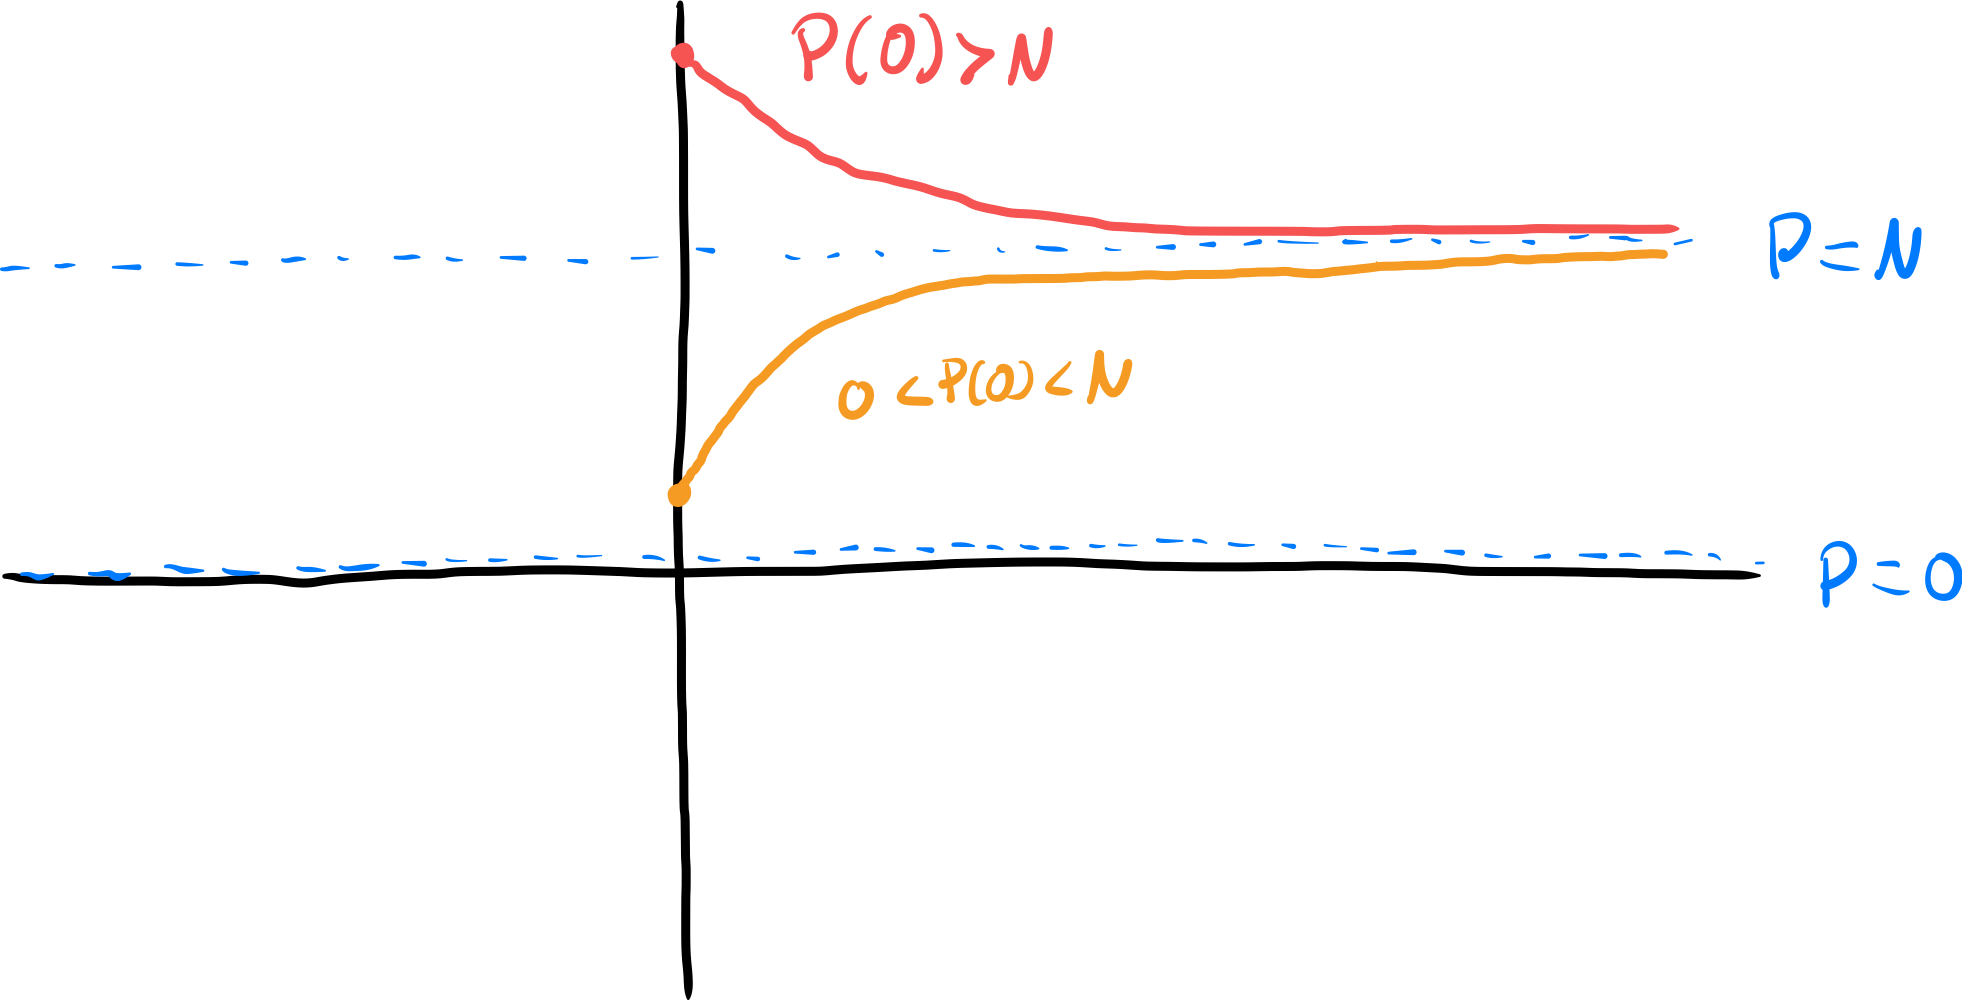
\includegraphics[width=10cm]{images/logistic_map.png}
    \end{center}
  \end{example}
\subsection{Separable First-Order Differential Equations}%
Consider the first-order differential equation
\begin{align*}
  \frac{dy}{dt} &= f(t,y).
\end{align*}
\begin{definition}[Separable Differential Equation]
  A differential equation of the form
  \begin{align*}
    \frac{dy}{dt} &= g(t)h(y)
  \end{align*}
  is called separable.
\end{definition}
\begin{note}
\begin{align*}
  f(t,y) = g(t)h(y).
\end{align*}
\end{note}
\begin{example}\hfill
  \begin{enumerate}[(1)]
    \item We can see that $\frac{dP}{dt} = kP$ is separable; $g(t) = k$, $h(y) = P$.
    \item We can see that $\frac{dy}{dt} = -\frac{t}{y}$ is also separable; $g(t) = -t$, $h(y) = \frac{1}{y}$.
    \item We can see that $\frac{dy}{dt} = y + t$ is not separable.
  \end{enumerate}
\end{example}
\begin{method}[Separation of Variables]
  We want to solve $\frac{dy}{dt} = g(t)h(y)$.
  \begin{enumerate}[(1)]
    \item We take $\frac{dy}{h(y)} = g(t)\:dt$ by multiplying $dt$ on both sides and dividing by $h(y)$.
    \item Integrate both sides with respect to their corresponding variable, yielding
      \begin{align*}
        \int_{}^{} \frac{1}{h(y)}\:dy &= \int_{}^{} g(t)\:dt.
      \end{align*}
    \item We get
      \begin{align*}
        H(y) &= G(t) + C,
      \end{align*}
      where $H(y)$ and $G(t)$ are antiderivatives of $\frac{1}{h(y)}$ and $g(t)$ respectively.
  \end{enumerate}
\end{method}
\begin{example}[Solving the Exponential Population Growth Model by Separation of Variables]
  Let $\frac{dP}{dt} = kP$, $P(0) = P_0$.
  \begin{align*}
    \frac{dP}{dt} &= kP\\
    \frac{dP}{P} &= k\:dt\\
    \int_{}^{} \frac{1}{P}\:dP &= \int_{}^{} k\:dt\\
    \ln|P| &= kt + C\\
    |P| &= e^{kt + C}\\
      &= e^{kt}e^{C}\\
    P &= \left(\pm e^{C}\right)e^{kt}\\
      &= Ae^{kt}.
  \end{align*}
  Our solution is now of the form $P(t) = Ae^{kt}$ (where $A = \pm e^{C}$). This is not the general solution, though, since it lacks our equilibrium solution of $P = 0$. Thus, the general solution is
  \begin{align*}
    \begin{cases}
      P(t) = Ae^{kt}\\
      P(t) = 0
    \end{cases}
  \end{align*}
  With the initial condition of $P(0) = P_0$, we have
  \begin{align*}
    P_0 = P(0)
         &= Ae^{k\cdot 0}\\
         &= A.
  \end{align*}
  Thus, the particular solution to our initial value problem is $P(t) = P_0e^{kt}$.
\end{example}
\begin{example}[Solving a Sample Differential Equation by Separation of Variables]
  Let $\frac{dy}{dt} = y^2 - 4$. Note that, even though this is not a linear equation, this is a separable equation. We start with the equilibrium solutions, which are at $y(t) = 2$ and $y(t) = -2$.\newline

  If $y\neq \pm 2$, we have
  \begin{align*}
    \frac{dy}{dt} &= y^2 - 4\\
    \frac{1}{y^2 - 4}\:dy &= dt\\
    \int_{}^{} \frac{1}{4(y-2)} - \frac{1}{4(y+2)}\:dy &= \int_{}^{} \:dt\\
    \frac{1}{4}\left(\ln\left|\frac{y-2}{y+2}\right|\right) &= t + C_1\\
    \ln \left\vert \frac{y-2}{y+2} \right\vert &= 4t + C_2\\
    \left\vert \frac{y-2}{y+2} \right\vert &= e^{C_2}e^{4t}\\
                                           &= C_3e^{4t}\\
    \frac{y-2}{y+2} &=  \pm C_3 e^{4t}\\
                    &= C e^{4t}\\
    y &= 2 + y Ce^{4t} + 2Ce^{4t}\\
    y &= \frac{2\left(1 + Ce^{4t}\right)}{1-Ce^{4t}}.
  \end{align*}
  Thus, our general solution is
  \begin{align*}
    \begin{cases}
     y(t) = \frac{2\left(1 + Ce^{4t}\right)}{1-Ce^{4t}} \\
     y(t) = 2\\
     y(t) = -2
    \end{cases}
  \end{align*}
\end{example}
\begin{example}[Solving the Logistic Population Growth Model]
  Let $\frac{dP}{dt} = kP\left(1-\frac{P}{N}\right)$. Our equilibrium solutions are at $P(t)=0$ and $P(t)=N$. For non-equilibrium solutions, we have
  \begin{align*}
    \frac{dP}{dt} &= kP\left(1-\frac{P}{N}\right)\\
    \frac{1}{P\left(1-\frac{P}{N}\right)}\: dP &= k\:dt\\
    \int_{}^{} \frac{1}{P\left(1-\frac{P}{N}\right)}\:dP &= \int_{}^{} k\:dt\\
    \int_{}^{} \frac{-N}{P\left(P-N\right)}\:dP &= kt + C_1\\
    \int_{}^{} \frac{1}{P} - \frac{1}{P-N}\:dP &= kt + C_1\\
    \ln \left\vert P \right\vert - \ln \left\vert P-N \right\vert &= kt + C_1\\
    \ln \left\vert \frac{P}{P-N} \right\vert &= kt + C_1\\
    \left\vert \frac{P}{P-N} \right\vert &= e^{C_1}e^{kt}\\
    \frac{P}{P-N} &= \pm e^{C_1}e^{kt}\\
                  &= Ce^{kt}\\
    P\left(1-Ce^{kt}\right) &= -NCe^{kt}\\
    P &= N\frac{Ce^{kt}}{Ce^{kt} - 1}.
  \end{align*}
  Therefore, our general solution is
  \begin{align*}
    \begin{cases}
      P(t) = N\frac{Ce^{kt}}{Ce^{kt} - 1}\\
      P(t) = 0\\
      P(t) = N
    \end{cases}.
  \end{align*}
\end{example}
\begin{example}[A Non-Separable Linear Differential Equation]
  Consider the linear differential equation
  \begin{align*}
    \frac{dy}{dt} + a(t) y &= b(t).
  \end{align*}
  Notice that
  \begin{align*}
    \frac{dy}{dt} &= -a(t)y + b(t),
  \end{align*}
  which is not able to be separated.\newline

  In order to solve such an equation, we will need to use an integrating factor.
\end{example}
\subsection{Slope Fields}%
\begin{definition}
  A slope field is a set of short line segments that indicate slope $\frac{dy}{dx}$ at a set of points $(x,y)$ in the $xy$ plane.\newline

  It is a graphical method of displaying the general slope and behavior of functions that satisfy $\frac{dy}{dx} = f(x,y)$.
\end{definition}
\begin{example}
  Consider $\frac{dy}{dx} = 1-y$. We can select some samples of slopes as follows:
  \begin{center}
    \begin{tabular}{c|c}
      Point & $\frac{dy}{dx}$\\
      \hline
      $(0,0)$ & $1$\\
      $(1,0)$ & $1$\\
      $(0,1)$ & $0$\\
      $(0,2)$ & $-1$
    \end{tabular}
  \end{center}
  Thus, we can draw the slope field:
  \begin{center}
    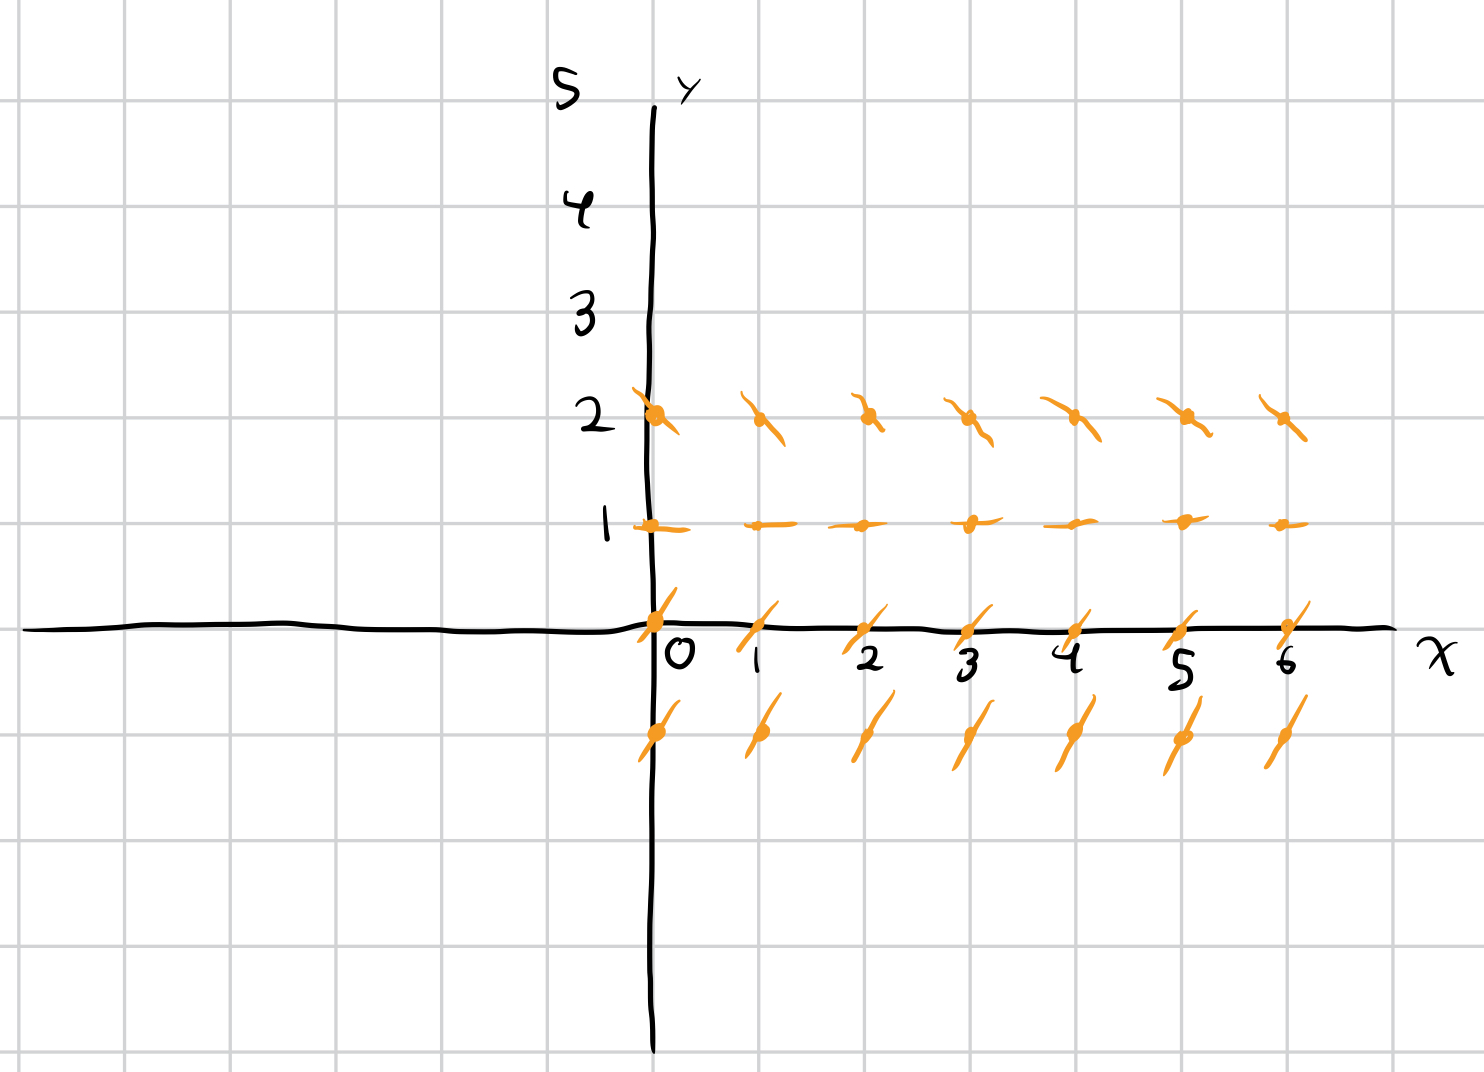
\includegraphics[width=7cm]{images/slope_field_2.png}
  \end{center}
  Qualitatively, we can see that
  \begin{itemize}
    \item at $y = 1$, all line segments are horizontal;
    \item for $y < 1$, all line segments have positive slope;
    \item for $y > 1$, all line segments have negative slope.
  \end{itemize}
  Using a computer, we can generate a better slope field:
  \begin{center}
    \begin{tikzpicture}
\begin{axis}[
  axis x line*=center,
  axis y line*=center,
	xmin = -4, xmax = 4,
	ymin = -4, ymax = 4,
	zmin = 0, zmax = 1,
	axis equal image,
    xtick={-4,-3,-2,-1,0,1,2,3,4},
    ytick={-4,-3,-2,-1,0,1,2,3,4},
	view = {0}{90},
]
	\addplot3[
    color=black!70!white,
		quiver = {
			u = {1/sqrt(1+(1-y)^2)},
			v = {(1-y)/sqrt(1+(1-y)^2)},
			scale arrows = 0.25,
		},
		-stealth,
		domain = -4:4,
		domain y = -4:4,
	] {0};
\end{axis}
\end{tikzpicture}
  \end{center}
  Analytically, we solve the equation by separation of variables:
  \begin{align*}
    \frac{dy}{dx} &= 1-y\\
    \frac{dy}{1-y} &= dx\\
    \int_{}^{} \frac{1}{1-y}\:dy &= \int_{}^{} \:dx\\
    -\ln|1-y| &= x + C\\
    \left\vert 1-y \right\vert &= e^{-x-C_1}\\
    1-y &= \pm e^{-C_1}e^{-x}\\
    y &= 1-Ae^{-x}.
  \end{align*}
  With the initial condition of $y(0) = -1$, we get $y = 1-2e^{-x}$.

  \begin{center}
    \begin{tikzpicture}
\begin{axis}[
  axis x line*=center,
  axis y line*=center,
	xmin = -4, xmax = 4,
	ymin = -4, ymax = 4,
	zmin = 0, zmax = 1,
	axis equal image,
	view = {0}{90},
    xtick={-4,-3,-2,-1,0,1,2,3,4},
    ytick={-4,-3,-2,-1,0,1,2,3,4},
]
	\addplot3[
    color=black!20!white,
		quiver = {
			u = {1/sqrt(1+(1-y)^2)},
			v = {(1-y)/sqrt(1+(1-y)^2)},
			scale arrows = 0.25,
		},
		-stealth,
		domain = -4:4,
		domain y = -4:4,
	] {0};
\addplot[
		-stealth,
		domain = -4:4,
    samples=250,
    color=red
    ]{1 - 2*pow(e,-x)};
\end{axis}
\end{tikzpicture}
  \end{center}
\end{example}
\subsection{Euler's Method}%
We want to approximate solutions to the differential equation $y' = f(x,y)$, $y(x_0) = y_0$. In the diagram, we can see the use of the slope field to calculate the approximate values of $\left(x_i,y_i\right)$.
\begin{center}
  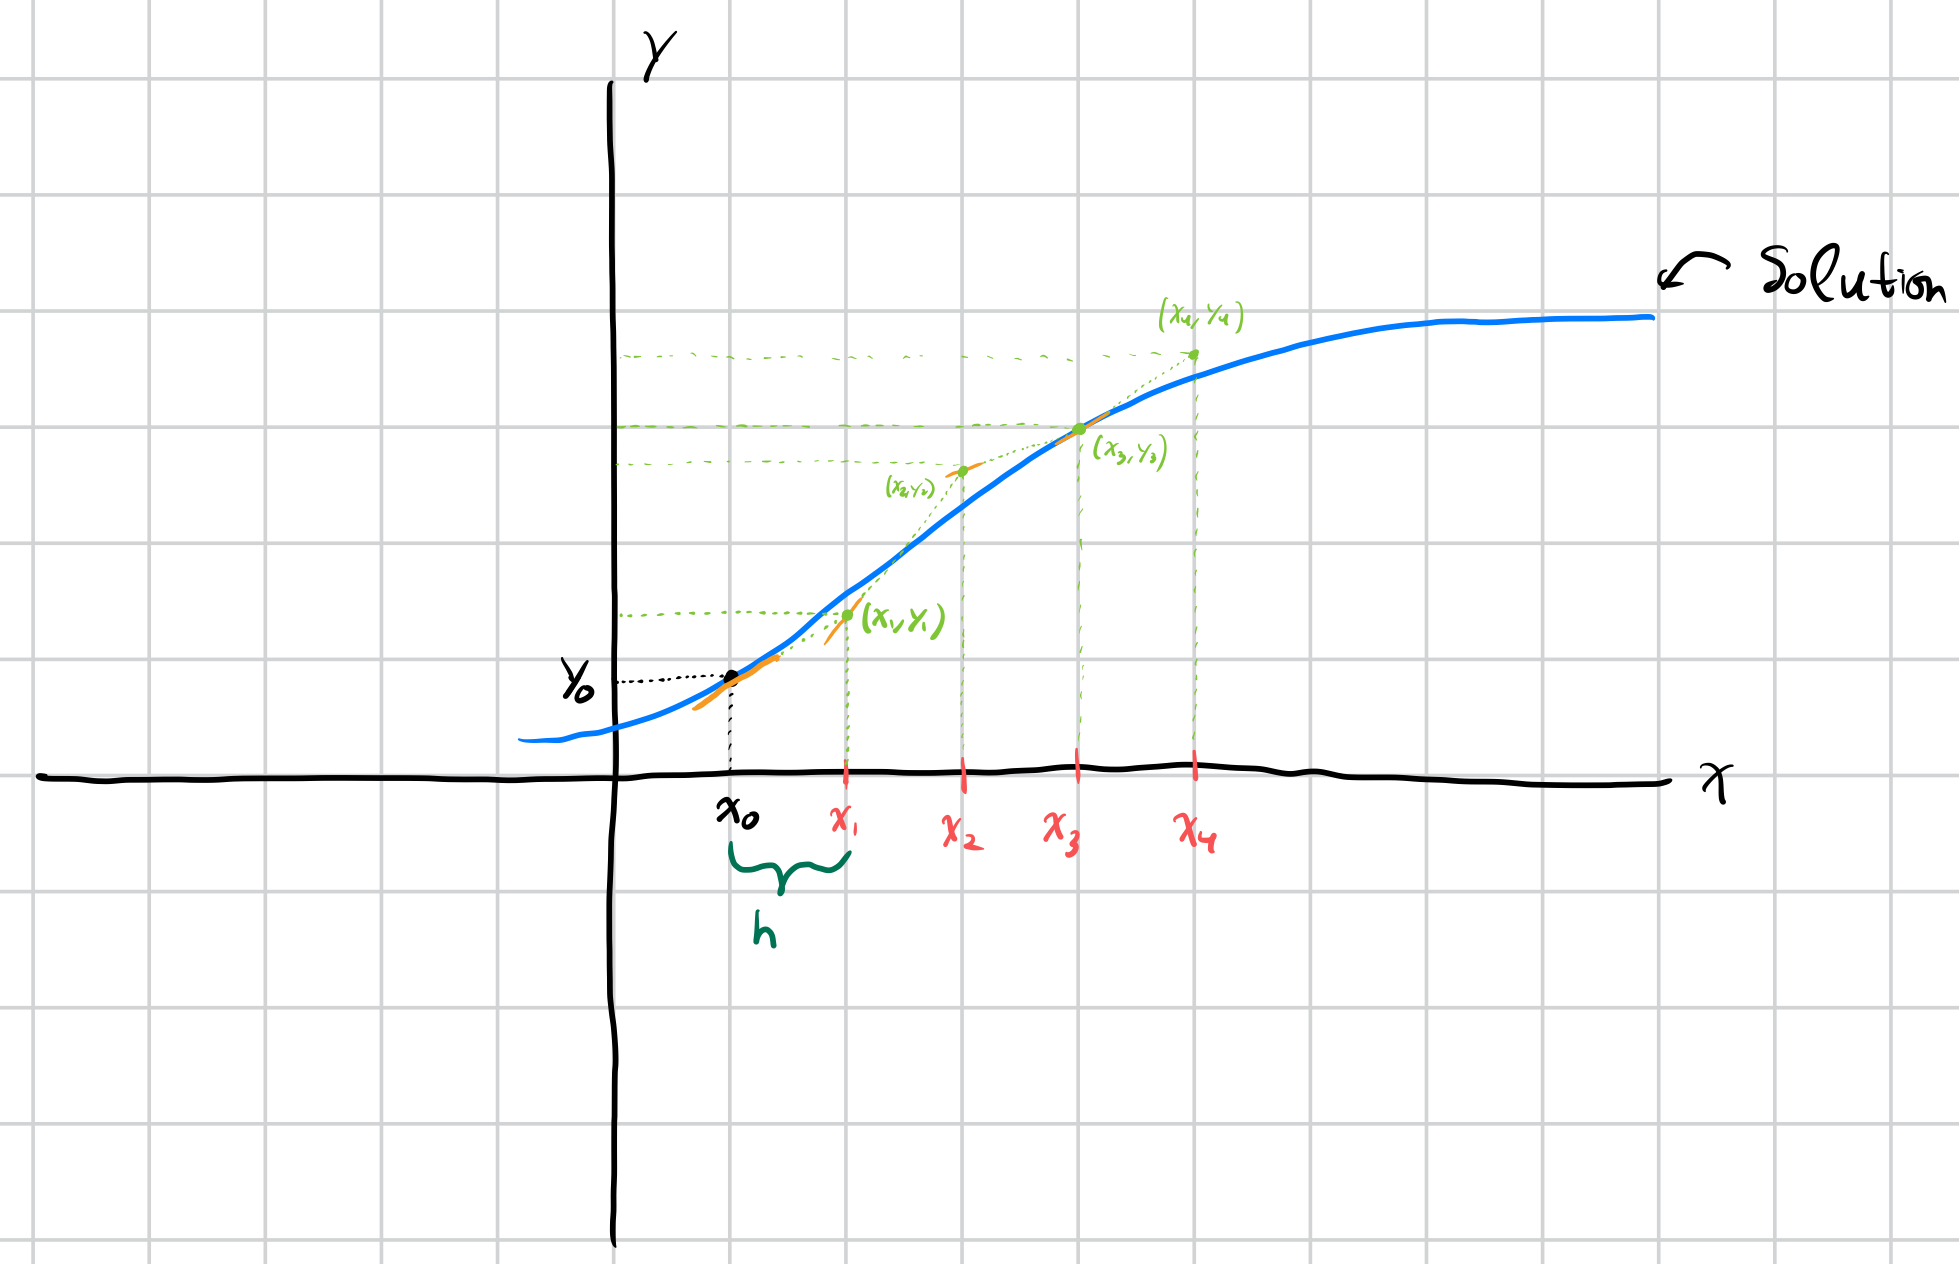
\includegraphics[width=15cm]{images/eulers_method_1.png}
\end{center}
\begin{method}[Euler's Method]
  To approximate the curve at $x_1 = x_0 + h$, we take the point-slope form:
  \begin{align*}
    \frac{y_1 - y_0}{\left(x_0 + h\right)-x_0} &= f\left(x_0,y_0\right)\\
    y_1 &= y_0 + hf\left(x_0,y_0\right).
  \end{align*}
  In general, we have
  \begin{align*}
    y_{n+1} &= y_k + hf\left(x_k,y_k\right).
  \end{align*}
\end{method}
\begin{example}
  Consider the differential equation $y' = 2y-1$. With the step size $\Delta x = h = 0.5$ and $y(0) = 1$, we can approximate $y(1)$ by
  \begin{center}
    \begin{tabular}{c|c|c|c}
      k & $x_k$ & $y_k$ & $f\left(x_k,y_k\right)$\\
      \hline
      $0$ & $1$ & 1 & 1\\
      $1$ & $1.5$ & $1.5$ & $2$\\
      $2$ & $2$ & $2.5$ & ---
    \end{tabular}
  \end{center}
  Thus, using Euler's method with a step size of $0.5$, we find that $y(1)\approx 2.5$. The table is read left to right, changing columns after calculating $f\left(x_k,y_k\right)$, then using it to calculate $y_{k+1}$.\newline

  Solving the differential equation analytically, we find
  \begin{align*}
    \frac{dy}{dx} &= 2y-1\\
    \int_{}^{} \frac{1}{2y-1}\:dy &= \int_{}^{} \:dx\\
    \frac{1}{2}\ln\left\vert 2y-1 \right\vert &= x + C_1\\
    \ln\left\vert 2y-1 \right\vert &= 2x + C_2\\
    \left\vert 2y-1 \right\vert &= e^{C_2}e^{2x}\\
    2y-1 &= \pm e^{C_2}e^{2x}\\
    y &= \frac{1}{2} + Ae^{2x}.
  \end{align*}
  Plugging in our initial condition, we find $A = \frac{1}{2}$, and the exact value of $y(1)$ is $\frac{1}{2} + \frac{1}{2}e^2$, which is approximately $4.1945$.\newline

  We can make our approximation via Euler's method better using a shorter step size.\newline

  For instance, by using a step size of 0.1, we find:
  \begin{center}
    \begin{tabular}{c|c|c|c}
      $k$ & $x_k$ & $y_k$ & $2y_k - 1$\\
      \hline
      $0$ & $0$ & $1$ & $1$\\
      1 & $0.1$ & $1.1$ & $1.2$ \\
      $2$ & $0.2$ & $1.22$& $1.44$ \\
      $3$ & $0.3$ & $1.364$& $1.728$\\
      $4$ & $0.4$ &$1.537$ & $2.07$\\
      $5$ & $0.5$ & $1.744$& $2.49$\\
      $6$ & $0.6$ & $1.993$ & $2.97$\\
      $7$ & $0.7$ & $2.29$ & $3.58$\\
      $8$ & $0.8$ & $2.65$ & $4.30$\\
      $9$ & $0.9$ & $3.08$& $5.16$\\
      $10$ & $1$ & $3.596$ & ---
    \end{tabular}
  \end{center}
  Note that our final approximation of $3.596$ is much better than the approximation under $h = 0.5$.\newline

  In order to understand if our estimate with Euler's method is an overestimate or underestimate, we use the second derivative test.
  \begin{align*}
    y' &= 2y - 1\\
    y'' &= 2y'\\
       &= 2\left(2y-1\right)\\
       &= 4y-2.
  \end{align*}
  In particular, our initial condition of $y(0) = 1$ suggests that $y'' = 2 > 0$, meaning Euler's method will return an underestimate (as the tangent lines will lie below the true curve).
\end{example}
\end{document}
